% Part: history
% Chapter: biographies
% Section: gerhard-gentzen

\documentclass[../../../include/open-logic-section]{subfiles}

\begin{document}

\olfileid{his}{bio}{gen}

\olsection{Gerhard Gentzen}

\begin{figure}[h!] 
\centering
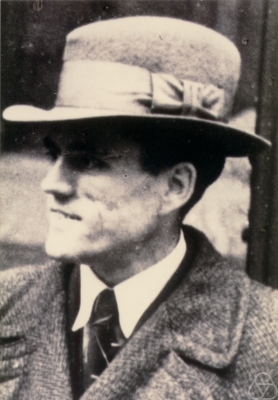
\includegraphics[scale=0.55]{gerhard-gentzen.jpg} 
\caption{Photo Credit: ``Gerhard Gentzen'' by Eckart Menzler-Trott}
\end{figure}

Gerhard Gentzen is known primarily as the creator of structural proof
theory, and specifically the creation of the natural deduction and 
sequent calclus proof systems. Gentzen was born on November 24, 1909 in 
Greifswald, Germany. Gerhard was homeschooled for three years before 
attending prepratory school, where he was behind most of his classmates in
 terms of education \citep[12]{Menzler-Trott2007}. Despite this, he was a
 brilliant student and showed a strong aptitude for mathematics. However,
it seems that his interests were varied, and he was known to write poems for 
his mother and plays for the school theatre \citep[11, 13]{Menzler-Trott2007}.

Gentzen began his university studies at the University of Greifswald, but
moved around to G\"{o}ttingen, Munich, and Berlin. He recieved his
doctorate in 1933 from the University of G\"{o}ttingen under Hermann Weyl,
after Paul Bernays was let go from his position at the university.
In 1934 he began work as an assistant to David Hilbert. That same year he
developed the sequent calculus and natural deduction proof systems, in his
papers \emph{Untersuchungen \"{u}ber das logische Schlie\ss en
I--II [Investigations Into Logical Deduction I--II]}. He proved the consistency
 of the Peano axioms in 1936.

The rise of Nazi power in Germany had a profound impact on Gentzen's life
and career. He swore an oath of Adolf Hitler as part
of his academic appointments \citep[119]{Menzler-Trott2007}.
In 1938 Gentzen joined the SA (the precursor to the SS) where he
worked as a telecommunications officer for the air intelligence
unit \citep[469]{Segal2014}. However, in 1942 he was released from duty due
to a nervous breakdown \citep[469]{Segal2014}. It is unclear whether or not
Gentzen's loyalties lay with the Nazi party, or whether he joined the party
 in order to ensure academic success.

In 1943, after being let go from his position with the SA, Gentzen was offered 
an academic position at the Mathematical Institute of the
German Univeristy of Prague, which he accepted. However, in 1945 the
citizens of Prague revolted against German occupation. Russian forces
arrived in the city and arrested all the professors at the univeristy.
Because of his work with the SA, Gentzen was taken to a forced labour camp. He
died of maltutrition while in his cell on August 4, 1945 at the age of 35.

\begin{reading}
\begin{itemize}
\item For a full biography of Gentzen, see \citet{Menzler-Trott2007}.

\item An interesting read about mathematicians under Nazi rule, which gives a
brief note about Gentzen's life, is given by \citet{Segal2014}.

\item Gentzen's papers have been collected in a single volume by 
\citet{Gentzen1969}, which also includes a biographical sketch.

\item Gentzen's original papers on logical deduction are available in the
original german \citep{Gentzen1935a,Gentzen1935b}, and in English 
translation \citep{Gentzen1969}.

\end{itemize}
\end{reading}

\end{document}
